\documentclass[a4paper]{report}

% Paquets généraux
\usepackage[utf8]{inputenc}     % Codage du fichier TeX
\usepackage[T1]{fontenc}        % Codage du fichier PDF (les paquets cm-super ou lmodern doivent être installés pour obtenir un bon résultat)
\usepackage{helvet}             % Police Helvetica
%\fontfamily{WalbaumGrotesk Text}
\usepackage{graphicx}           % Logos et autres illustrations
%\usepackage{fancyhdr}           % En-têtes et pieds de page
\usepackage{color}              % Couleur
\usepackage{ifthen}             % Condition

\usepackage[french]{babel}      % Courrier en français

\usepackage[colorinlistoftodos]{todonotes}
\usepackage{url}
%pour les informations sur un document compilé en PDF et les liens externes / internes
\usepackage{hyperref}

%pour la mise en page des tableaux
\usepackage{array}
\usepackage{tabularx}

% Papier à en-tête ICube
% Version du 3 février 2013
% Infos et bugs : vincent.mazet@unistra.fr

% Mise en page
\voffset -1in
\topmargin 10mm
\headheight 5mm
\headsep 35mm
\textheight 210mm
\footskip 20mm
\hoffset -1in
\oddsidemargin 50mm
\evensidemargin 50mm
\textwidth 140mm
\marginparsep -180mm
\marginparwidth 35mm
\parindent 0mm


% Police sans-serif
\renewcommand{\familydefault}{\sfdefault}

% Couleurs
\definecolor{vert}{RGB}{15.3,63.5,17.6}
\definecolor{gris}{RGB}{88,88,90}

% Logos
%\newcommand{\icubesign}{\includegraphics[width=40mm]{icube-sign.eps}\vspace*{-20mm}}
\newcommand{\logoCirad}{
\includegraphics[width=40mm]{logo/logo-cirad-fr.jpg}\vspace*{-20mm}}
%\newcommand{\icube}{
\includegraphics[width=40mm]{Republique-francaise-logo.png}\vspace*{-12mm}}
\newcommand{\logoRF}{
\includegraphics[width=40mm]{logo/Republique-francaise-logo.png}\vspace*{-12mm}}
\newcommand{\partnerFr}{
\includegraphics[width=40mm]{logo/partner-with-france.jpg}\vspace*{-12mm}}
             % Style de la lettre à en-tête

%espacement entre les lignes
\usepackage{setspace}
%modifier la mise en page de l'abstract
\usepackage{abstract}

%Pour les galerie d'images
\usepackage{subfig}

%====================== INFORMATION ET REGLES ======================

%rajouter les numérotation pour les \paragraphe et \subparagraphe
\setcounter{secnumdepth}{4}
\setcounter{tocdepth}{4}

\hypersetup{							% Information sur le document
pdfauthor = {Premier Auteur,
			Deuxième Auteur,
			Troisième Auteur,
    		Quatrième Auteur},			% Auteurs
pdftitle = {Nom du Projet -
			Sujet du Projet},			% Titre du document
pdfsubject = {Mémoire de Projet},		% Sujet
pdfkeywords = {Tag1, Tag2, Tag3, ...},	% Mots-clefs
pdfstartview={FitH}}					% ajuste la page à la largueur de l'écran
%pdfcreator = {MikTeX},% Logiciel qui a crée le document
%pdfproducer = {}} % Société avec produit le logiciel


\begin{document}

%régler l'espacement entre les lignes
\newcommand{\HRule}{\rule{\linewidth}{0.5mm}}

%page de garde
\begin{titlepage}
\begin{center}

% Upper part of the page. The '~' is needed because only works if a paragraph has started.
\logoCirad ~ 
\includegraphics[height=30mm]{./logo/cnrs.png} ~ 
\includegraphics[height=30mm]{./logo/ign.png}\\[6cm]

%\textsc{\LARGE Université ou Entreprise}\\[1.5cm]

\textsc{\Large }\\[0.5cm]

% Title
\HRule \\[0.4cm]
\includegraphics[height=30mm]{./logo/DSCATT.png}\\
{\huge \bfseries Rapport intermediaire \\
 Comment se maintient la jachère communautaire de Diohine ? \\[0.4cm] }

\HRule \\[1.5cm]


% Author and supervisor
\begin{minipage}{0.4\textwidth}
\begin{flushleft} \large
\emph{\textcolor{gris}{Auteur:}}\\
Etienne \textsc{Delay}\\
\textcolor{vert}{CIRAD Dir ES. UMR SENS}\\
\vfill{2em}
Paul \textsc{Chapron} (IGN)\\
Romain \textsc{Reuillon} (CNRS)\\
Mathieu \textsc{Leclaire} (CNRS)
\end{flushleft}
\end{minipage}
\begin{minipage}{0.4\textwidth}
\begin{flushright} \large
\emph{\textcolor{gris}{Chef de Projet:}} \\
Abigail \textsc{Fallot} - CIRAD\\
Dominique \textsc{Masse} - IRD
%\textcolor{vert}{GRET}
\end{flushright}
\end{minipage}

\vfill

\logoRF ~ \partnerFr
% Bottom of the page
{\large \today}

\end{center}
\end{titlepage}


%page blanche
\newpage
~
%ne pas numéroter cette page
\thispagestyle{empty}
\newpage

\renewcommand{\abstractnamefont}{\normalfont\Large\bfseries}
%\renewcommand{\abstracttextfont}{\normalfont\Huge}

\begin{abstract}
\hskip7mm

\begin{spacing}{1.3}

Lorem ipsum dolor sit amet, consectetur adipiscing elit. Sed non risus. Suspendisse lectus tortor, dignissim sit amet, adipiscing nec, ultricies sed, dolor. Cras elementum ultrices diam. Maecenas ligula massa, varius a, semper congue, euismod non, mi. Proin porttitor, orci nec nonummy molestie, enim est eleifend mi, non fermentum diam nisl sit amet erat. Duis semper. Duis arcu massa, scelerisque vitae, consequat in, pretium a, enim. Pellentesque congue. Ut in risus volutpat libero pharetra tempor. Cras vestibulum bibendum augue. Praesent egestas leo in pede. Praesent blandit odio eu enim. Pellentesque sed dui ut augue blandit sodales. Vestibulum ante ipsum primis in faucibus orci luctus et ultrices posuere cubilia Curae; Aliquam nibh. Mauris ac mauris sed pede pellentesque fermentum. Maecenas adipiscing ante non diam sodales hendrerit. Ut velit mauris, egestas sed, gravida nec, ornare ut, mi. Aenean ut orci vel massa suscipit pulvinar. Nulla sollicitudin. Fusce varius, ligula non tempus aliquam, nunc turpis ullamcorper nibh, in tempus sapien eros vitae ligula. Pellentesque rhoncus nunc et augue. Integer id felis. Curabitur aliquet pellentesque diam. Integer quis metus vitae elit lobortis egestas. Lorem ipsum dolor sit amet, consectetuer adipiscing elit. Morbi vel erat non mauris convallis vehicula. Nulla et sapien. Integer tortor tellus, aliquam faucibus, convallis id, congue eu, quam. Mauris ullamcorper felis vitae erat. Proin feugiat, augue non elementum posuere, metus purus iaculis lectus, et tristique ligula justo vitae magna. Aliquam convallis sollicitudin purus. Praesent aliquam, enim at fermentum mollis, ligula massa adipiscing nisl, ac euismod nibh nisl eu lectus. Fusce vulputate sem at sapien. Vivamus leo. Aliquam euismod libero eu enim. Nulla nec felis sed leo placerat imperdiet. Aenean suscipit nulla in justo. Suspendisse cursus rutrum augue. Nulla tincidunt tincidunt mi. Curabitur iaculis, lorem vel rhoncus faucibus, felis magna fermentum augue, et ultricies lacus lorem varius purus. Curabitur eu amet.

\end{spacing}
\end{abstract}


\tableofcontents
\thispagestyle{empty}
\setcounter{page}{0}
%ne pas numéroter le sommaire

\newpage

%espacement entre les lignes d'un tableau
\renewcommand{\arraystretch}{1.5}

%====================== INCLUSION DES PARTIES ======================

~
\thispagestyle{empty}
%recommencer la numérotation des pages à "1"
\setcounter{page}{0}
\newpage

\chapter{Présentation du projet}

Intro\footnotemark\\
%note en bas de page

\section{Sujet}

%inclusion d'une mage dans le document
\begin{figure}
\begin{center}
%taille de l'image en largeur
remplacer "width" par "height" pour régler la hauteur

\includegraphics[width=15cm]{logo/GRET_logo}
\end{center}
%légende de l'image
\caption{Schéma descriptif}
\label{Tux}
\end{figure}

%Contenu de la note précédemment marquée avec \footnotemark
\footnotetext{Note bas de page "intro"}

Bla
%retour à la ligne (alinea)

Bla\\
%saut de paragraphe

Bla

\newpage



Auteurs : Paul Chapron (IGN), Romain Reuillon (ISCPIF), Mathieu Leclaire (ISCPF), Etienne Delay (CIRAD)

Pour le réaliser, on s'appuie sur deux notes : 
- Note de [Paul]\url{https://hackmd.openmole.org/Rck70wm6Qmu_ztM0M03--w?view}
- Note d'[Etienne]\url{https://hackmd.openmole.org/qhPAjsJGRbiOQYIItbwPww#}


:::info
public visé par le rapport : 

A minima les 4 acteurs (Paul, Marcel ,  Marie-Hélène et Idrissa), + toute personne intéressée par la zone de Diohine et sa spécificité : la gestion collective de l’espace à travers la survivance des jachères communautaire.

On n'hésitera pas a mettre des référence bilio
:::


\section{Contexte}

Dans le cadre du projet DSCATT, nous Paul Chapron (IGN) Romain Reuillon (CNRS) et Etienne Delay (CIRAD) avons animé 1 semaine d'atelier à Diohine sur le territoire de l'observatoire IRD de Niakhar. Ils s'inscrivent dans différentes réflexions de recherche autour de l'exploration d'accompagnement, et les théories de la viabilité appliquées aux systèmes multi-agents.
Ces journées d'atelier ont mobilisé quatre acteurs locaux sur cinq jours: 
- Paul Sene +221 77 623 60 93
- Marcel Latyr Diouf +221 77 198 41 06
- Marie Hélène Ndjira +221 77 072 57 60
- Idrissa Faye +221 77 408 24 76
- Robert Diate 

L'enjeu de cette semaine d'atelier était de formaliser avec les acteurs leur représentation du système d'interaction et de solidarité dans lequel s'inscrit la gestion collective de l'espace à travers la survivance des jachères communautaire. Le système de jachère est lui-même considéré comme un élément clef des processus de maintien de la fertilité des sols et donc un proxy sur les questions de stockage de carbone dans les sols. 

À l'issue de la semaine, les participants ont pu valider une première version de leur système qu'on retrouve ici : https://github.com/ElCep/DSCATT/tree/master/PARDi

\section{PARDi, un outil de mise en lumière de l'agencement des éléments du système.}

\subsection{Le diagramme  comme outil de représentation du système}

La méthode PARDI est une évolution des spécifications de ARDI (Etienne et al. 2011) qui relève de la capacité de l'outil à expliciter des implicites et rendre visible des  hypothèses de modélisation. Cette méthode mobilise des diagrammes pour représenter à la fois les éléments constitutifs du système et les interactions entre ces éléments. 

Ces diagrammes sont constitués de noeuds représentés par des cercles ou des ellipses, et d'arcs, représentés par des flèches, qui relient les noeuds. 

Dans un diagramme PARDI comme ceux que nous allons inclure dans la suite de ce rapport, les noeuds représentent des acteurs ou des ressources, et les arcs représentent des interactions entre ces acteurs, entre ces ressources ou entre ces acteurs et ces ressources.

%inclusion d'une mage dans le document
\begin{figure}
\begin{center}

\includegraphics[width=5cm]{img/diagramme_simple.png}
\end{center}
%légende de l'image
\caption{Interaction simple }
\label{simple_interac}
\end{figure}



Comme les noeuds et les arcs sont nommés, il devient facile de faire une phrase qui décrit l'interaction de façon concise. Par exemple avec la figure \ref{simple_interac} , on pourrait former la phrase suivante : « A consomme B»

Plusieurs arcs peuvent exister entre deux mêmes noeuds, pour représenter des interactions différentes.


\subsection{Modélisation PARDI du système de Diohine}

\subsubsection{Les Acteurs}

Par la suite nous utiliserons les termes suivants:
\begin{itemize}
\item \textbf{acteur/role}: personne physique partie prenante dans le système étudié
\item \textbf{participant} : personnes physiques concourant à la co-construction du modèle durant l'atelier. C'est donc un sous ensemble des "acteurs".
\end{itemize}

\vspace{0.5cm}

La méthode PARDI propose d'interroger des participants évoluant dans un même système. Ils participent à co-construire un diagramme d'interactions entre acteurs sur la base de la connaissance qu'ils ont de ce système. Elle a pour effet de les faire réfléchir sur la réalité du système dans lequel ils évoluent. Les échanges de points de vue stimulent leur créativité en mettant en lumière des liens entre certains objets de leurs quotidiens. L'enjeu du travail de modélisation conceptuel avec PARDI est d'accompagner par un mode de représentation schématique la réflexion sur le fonctionnement du système (Becu et al. 2010).\\


Les acteurs représentés dans le modèle sont:
\begin{itemize}
\item Agriculteur: paysan travaillant la terre et produisant de l'arachide et du mil.
\item Pasteur: éleveur utilisant les jachères comme pâturage pour son bétail
\item Chef de cuisine: homme ayant la responsabilité de nourrir tout ou partie de la famille.
\item Chef de concession (ou chef de famille): homme ayant la charge de la paix sociale au sein de la famille, et donc des différentes cuisines qui la compose.
\item Notable: personne importante dans le village (ex: instituteur, médecin, imam, etc)
\item Vieille maman:  femme agée, sage, capable 
\item Chef de village : autorité coutumière du lieu de peuplement, reconnu par l'autorité centrale de l'état. 
\item Conseil municipale : ensemble d'individus qui sont élus aux élections locales et qui s'insèrent dans le droit positif et les institutions de l'état.
\item Sous-préfet : Représentant de l'état décentralisé sur les territoires. Il prend en charge les conflits quand le droit traditionnel n'a pas réussi à trouver une solution convenable pour les différentes parti du conflit.
\item Saltigué : voyant et devin qui officie lors de la cérémonie divinatoire de la première chasse. Ses prédictions portent sur la météo, les catastrophes et les remèdes pour y faire face. Un saltigué a un quartier sous sa juridiction
\item Banque de Céréales : Structure locale (à l'échelle d'un quartier) qui prête des céréales aux agro-pasteurs contre une remboursement ultérieur et vend des céréales. Chaque cuisine contribue au stock de la banque.
\end{itemize}

Les acteurs ci-dessous ne nécessitent pas d'explicitation approfondie, leur nom étant assez explicite.

\begin{itemize}
\item École
\item Revendeur de semence
\item Revendeur d'engrais
\item Animal de trait : âne et cheval
\item Petit ruminant : mouton et chèvre
\item Grand ruminant : boeuf et vache
\end{itemize}

\subsubsection{L'atelier de modélisation PARDI à Diohine }

Dans le cadre du questionnement autour du stockage de carbone dans les pratiques agricoles du projet DSCATT, nous nous sommes intéréssés à la gestion communautaire de la jachère dans la commune de Diohine. 

La jachère est la pratique agricole visant à laisser au repos une parcelle entre deux cultures, généralement sur une période d'un an. À Diohine, cette jachère s'intercale la plupart du temps au sein d'un assolement triénal: Mil, Arachide, Jachère.

Ainsi la jachère a le double avantage de maintenir une fertilité élevée et de stocker du carbone. Ainsi s'intéresser au maintien d'une jachère gérée en commun à l'échelle d est un proxy du stockage de carbone tout en permettant à la population de subvenir à ses besoins alimentaires.

L'atelier de modélisation réunit:
- deux agro-pasteurs
- un agriculteur
- une agri-pastrice vieille maman 

Ils participent à co-construire le diagramme d'interaction d'un système agro-pastoral à l'échelle de la ville de Diohine, tentant de répondre à la problématique que nous pouvons formuler de la mamnière suivante : «Comment se maintient la jachère communautaire de Diohine ?»

Cette question fait suite à une première consultation à Diohine en mai 2021 lors de laquelle une inquiétude doublée d'une aspiration très forte a été formulée (voir figure \ref{aspiration}) : Comment préserver la jachère communautaire à Diohine ? (Perrotton *et al.* 2021) 

²Or, pour entrevoir comment préserver cette jachère communautaire à l'avenir, nous devons d'abord nous intéresser à ce qui fonde son existence; et c'est à cette question que nous allons nous intéresser dans les pages suivantes. 


Aussi pouvons-nous reformuler cette question en termes plus académiques et généraux de la façon suivante :  
Comment préserver une gestion foncière concertée de la fertilité ?

::: info
futur titre de la publication scientifique : 

Comment préserver une gestion foncière concertée de la fertilité ? : la survivance de la jachère communautaire de Diohine
:::


\begin{figure}
\begin{center}
%taille de l'image en largeur
remplacer "width" par "height" pour régler la hauteur
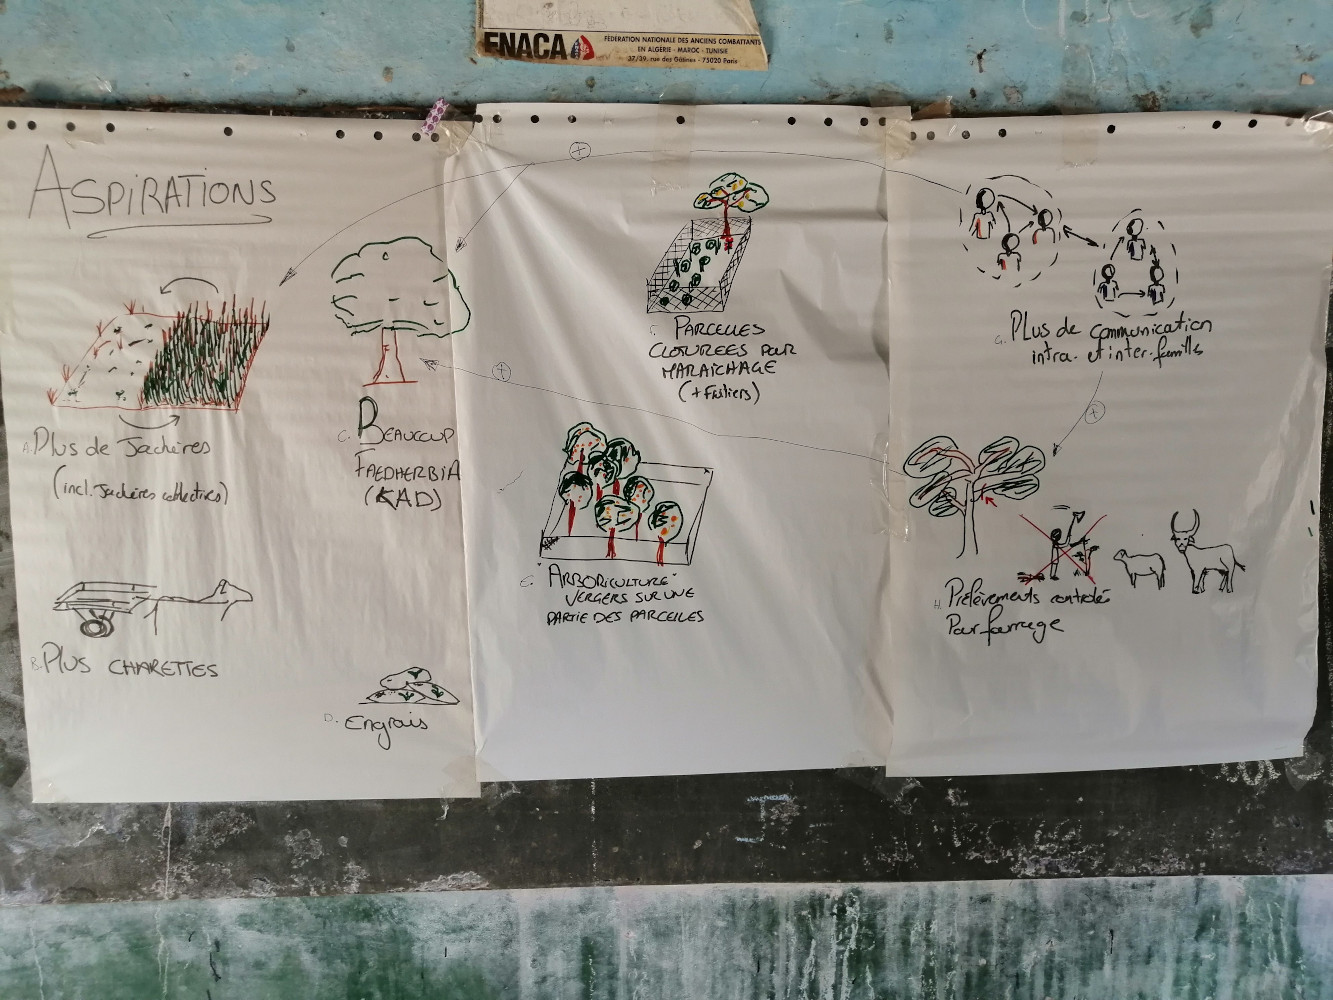
\includegraphics[width=15cm]{img/aspiration_formulee.jpg}
\end{center}
%légende de l'image
\caption{Interaction simple }
\label{aspiration}
\end{figure}





Le travail de modélisation a amené les participants à définir une centaine de nœuds et leurs arcs. Le diagramme complet est visible sur la figure \ref{diag_complet} 


\begin{figure}
\begin{center}
%taille de l'image en largeur
remplacer "width" par "height" pour régler la hauteur
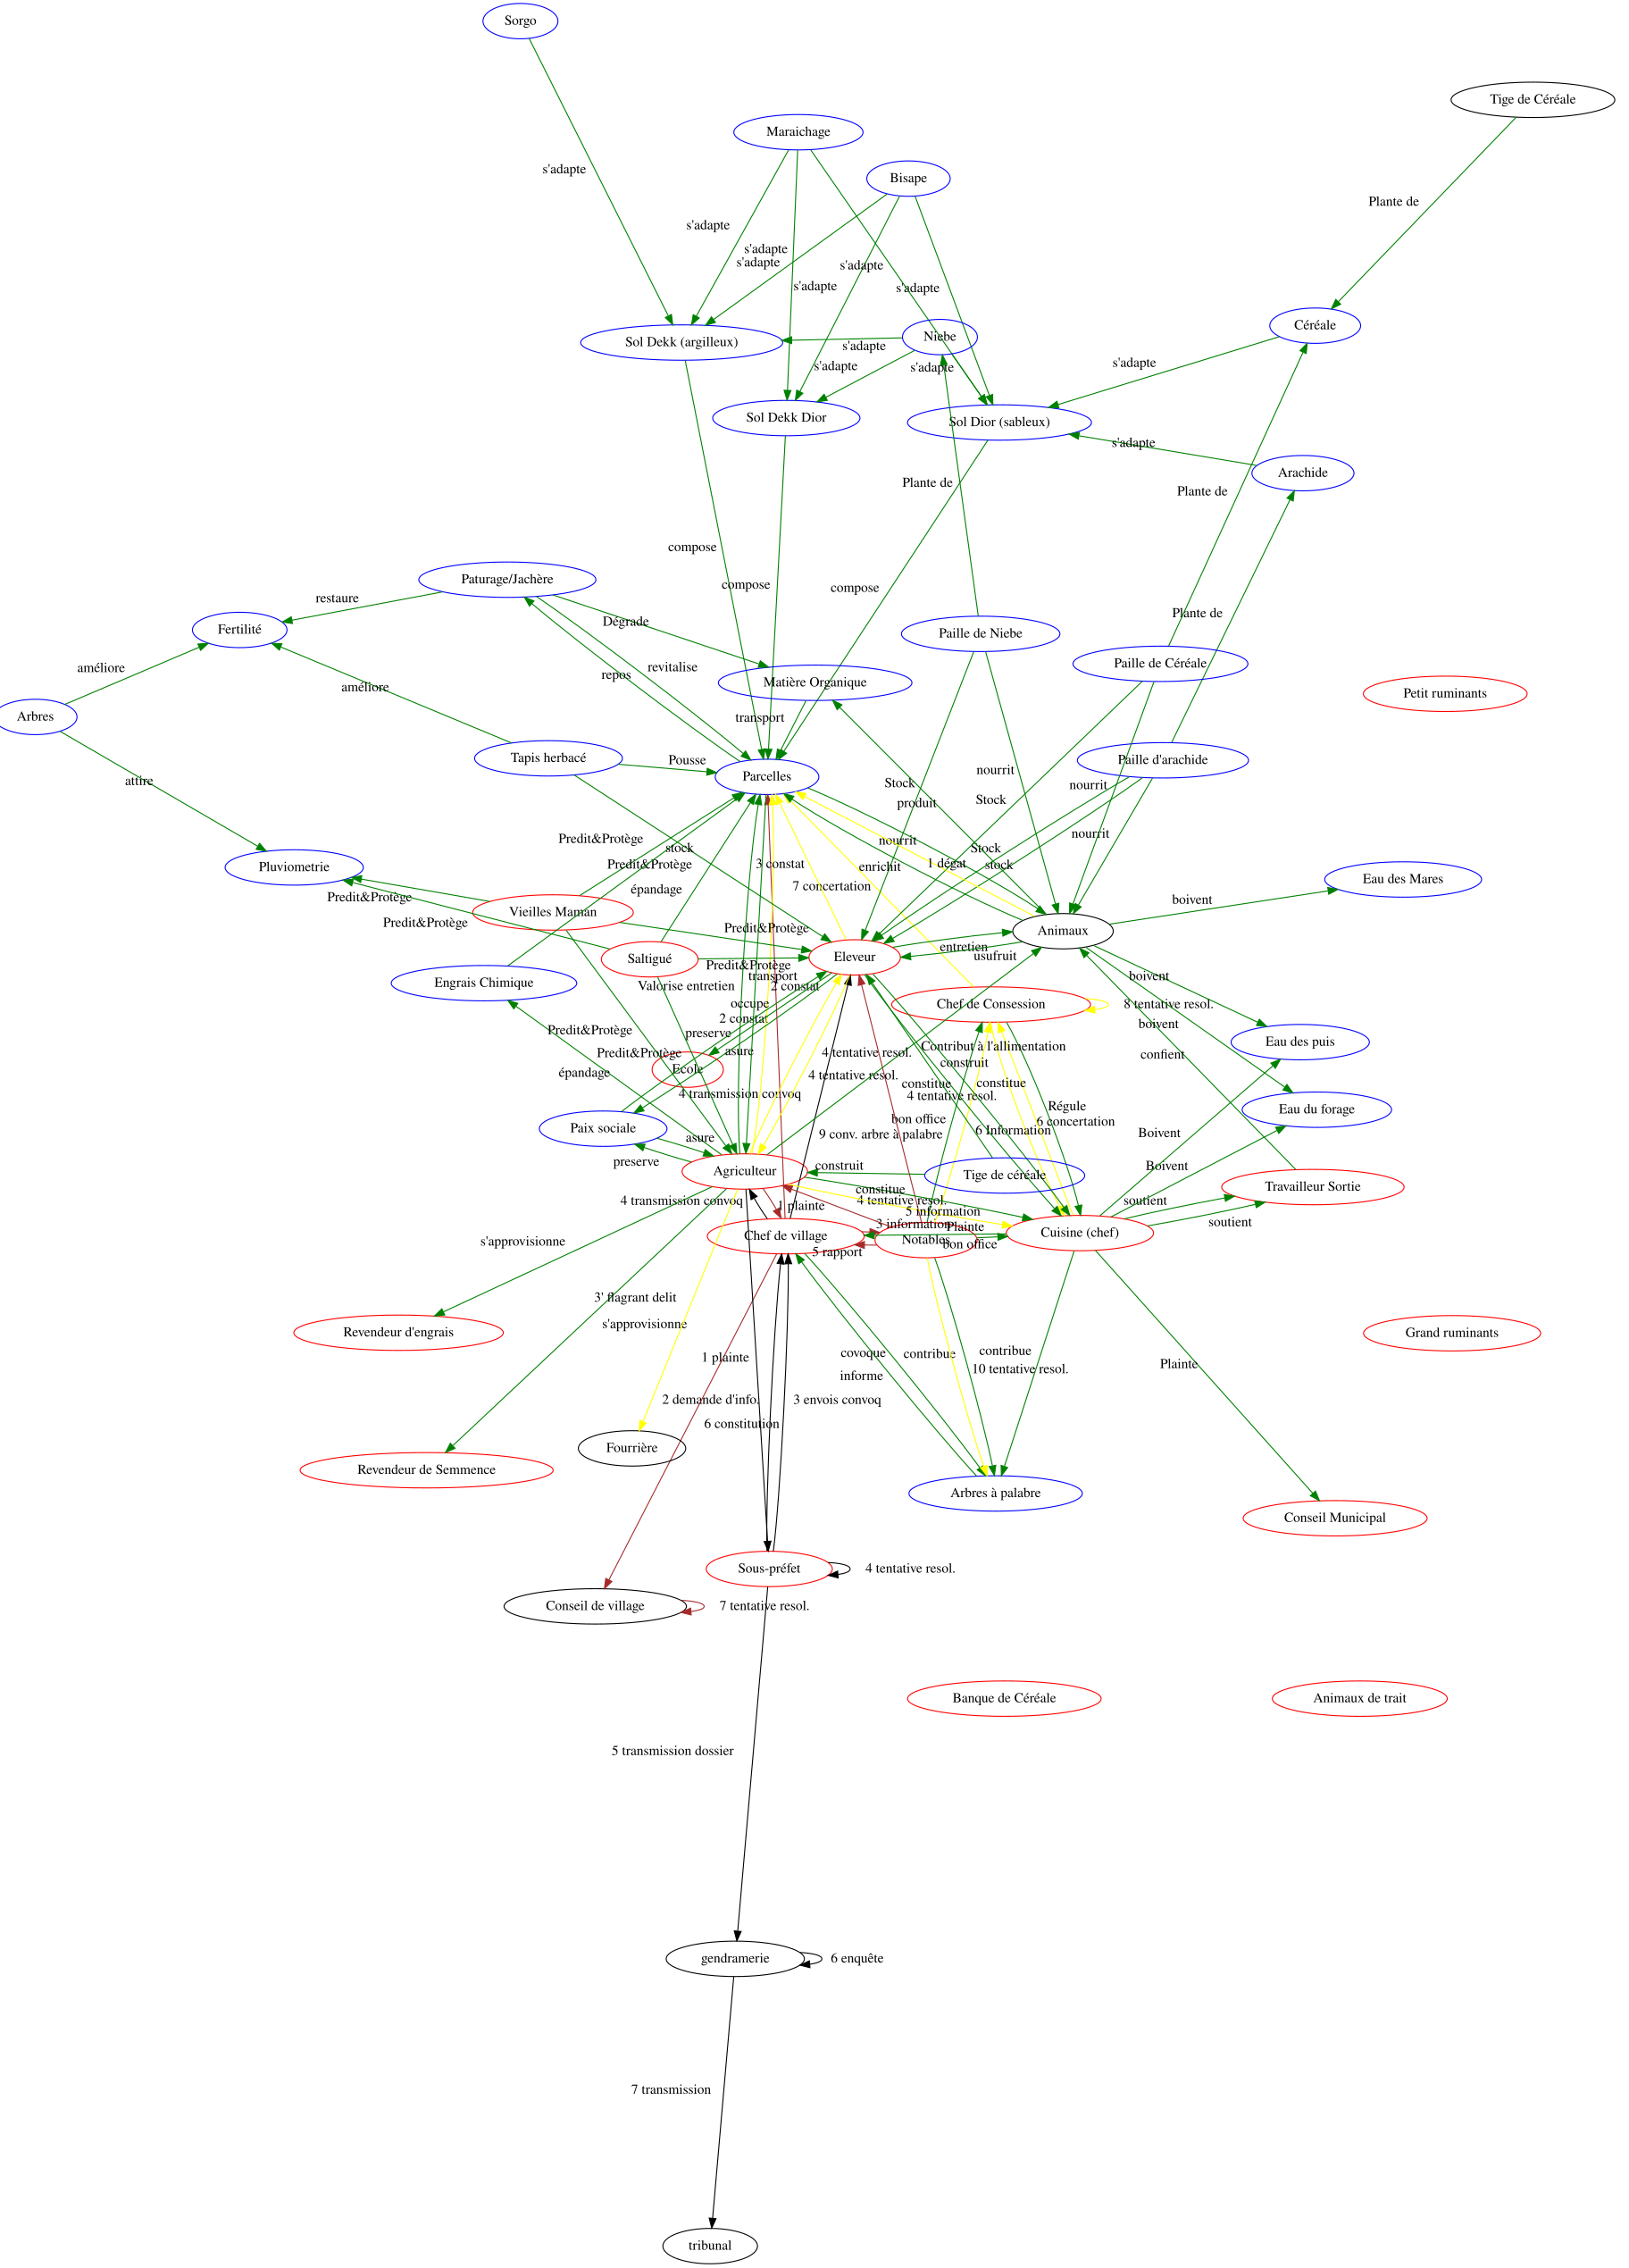
\includegraphics[width=15cm]{img/pardi_fdp.png}
\end{center}
%légende de l'image
\caption{Diagramme complet des interactions relevées pendant l'atelier à Diohine }
\label{diag_complet}
\end{figure}




Nous avons choisi de le restituer dans ce rapport avec quatre points de vue différents : 
1. les activités liées au rôle d'agro-pasteur
2. les mécanismes de résolution de conflit
3. les interactions liées à la gestion collective de l'espace
4. les réseaux de solidarités


\section{Conclusion}

Le territoire fait face à un phénomène d’éclatement des cuisines. Le concept de cuisine regroupe les personnes qui mangent ensemble et donc qui participent à l’alimentation. Du fait de l’imbrication des systèmes de solidarité (et du lien avec la lignée maternelle?)([paul] casse gueule la lignée ici) , la propension des acteurs à participer à l’alimentation de la cuisine est réduite aux obligations. Pour nos participants, les femmes participent très fortement à l’éclatement des cuisines.

«Avec l’éclatement des cuisines, il y a de moins en moins de place pour les fainéants. Tout le monde doit travailler à fond. »


Le prêt de terre est historiquement accompagné d’un cadeau en nature, mais aujourd’hui, cette pratique évolue vers de la location.

«Il y a de la solidarité en face de l’insuffisance»
En cas de maladie d’un paysan, le village se mobilise pour cultiver et récolter.
De la nourriture est glissée sous la porte, les greniers sont remplis de nuit , sans le dire.
la discrétion est importante


\section{Biblio pour le moment , à refaire en latex}

Becu, N., Bommel, P., Botta, A., Le Page, C., Perez, P., 2010. Les téchnologies mobilisées pour l’accompagnement, in: Etienne, M. (Ed.), La modélisation d’accompagnement une démarche participative en appui au développement durable. Quae éditions, Versailles, pp. 183–201.

Etienne, M., Du Toit, D., Pollard, S., 2011. ARDI: A Co-construction Method for Participatory Modeling in Natural Resources Management. Ecology and Society 16. [https://doi.org/10.5751/ES-03748-160144](https://doi.org/10.5751/ES-03748-160144)

----

\section{ Fin du document }

----

\subsection{ TODO sur le DOT}



- ouvrir le .dot dans R avec sna -> enregistrer en `.gv` on l'ouvre tout seul dans Rstudio. 
%[La doc de rendu est pas mal](https://rich-iannone.github.io/DiagrammeR/graphviz_and_mermaid.html)
- enrichir le graphe avec des attributs dans R ou à la main dans le fichier en utilisant la synthaxe de DiagrammR. par exemple `@@1` pour définir un attribut 
- visualiser avec diagrammeR
- Pour le rendu : utilisation de la substitution de diagrammeR pour changer les couleurs les formes etc.  des noeuds et des arêtes

\subsection{ Le workflow}
- Defintion de class de noeud
- Extrait les sous graph avec igraph
- enrichissemement des attribut du graph genre color etc.
renvoyer en `.gv`

Pour chaque sous graphe du graphe PARDI 

-  griser les noeuds non-impliqués dans un sous-graphe de façon à conserver la topologie/spatialisation du gros graphe et ne faire apparaître que les noeuds impliqués dans le sous-système



\section{TODO rédaction du texte }

\subsection{TODO GRAPHE}

\subsection{ TODO }

Typologie de trois catégories : une par sous graphe 

Rassembler les éléments du terrain (notes, souvenirs , soit la biblio , soit l'expérience perso) dans chacun des trois sous graphe.

Rédiger de façon descriptive

Enrichir/Augmenter la description avec de l'analytique  : caractérisation des processus (e.g. Ici les acteurs mobilisent leur capital social), des postures des acteurs, des résultats de l'action collective 


Illustrations diverses

Meta-discours : contextualisation , intro , conclusion et des encarts sur des termes spécifiques pour se faire bien comprendre par tous (e.g. Saltigué et stygmergie sont deux termes qu'il sera bon d'expliciter à tous )






\subsection{Journal de bord du modèle de simulation}


\subsubsection{Note pour un jour}
 - Les lois en droit positif on l'oublie trop souvent servent à maintenir la paix sociale.
 - Spinoza pose en effet qu'il suffit de ne pas comprendre pour moraliser. Et c'est ce à quoi servent les lois. À gérer les problèmes des gens qui ne veulent pas comprendre. "Si Adam ne comprend pas la règle du rapport de son corps avec le fruit, il entend la parole de Dieu comme une défense. Bien plus, la forme confuse de la loi morale a tellement compromis la loi de la nature que la philosophie ne doit pas parler de loi de la nature, mais seulement de vérité éternelles "  p. 35, "les lois morale ou sociale ne nous apportent aucune connaissance, elle ne fait rien connaitre". Au pire elle empêche la formation de la connaissance (loi des tyrans). Au mieux elle prépare la connaissance et la rend possible (loi d'Abraham). Entre ces deux extrêmes, elle supplée à la connaissance chez ceux qui n'en sont pas capables en raison de leurs modes d'existence (loi de moise)."
>[name= Etienne] J'ai l'impression que tout le système traditionnel à Diohine est tourné vers une résolution de conflit où la seule chose qui est donnée aux acteurs c'est des indications de posture (tu ne dois pas faire de tort...-> injonction morale/ethique -> ligne de conduite serere), Donc on les pousse à comprendre la source du conflict (mauvais de Spinoza)parce qu'il y a une injonction a l'action (une action de réparation). 
>
 Changement de plan/d'arène juridique : Quand ils ne sont pas parvenus à une résolution locale du conflit, on entre dans le droit positif (dur et sans empathie -> paul Sene) et là il y a des lois qui font qu'on a plus besoin de comprendre le source du mauvais.--> un lien avec un verbatim en [J4](\url{https://hackmd.openmole.org/qhPAjsJGRbiOQYIItbwPww#J4---21-octobre}) "Tout le processus est là pour éviter la dureté des lois. “*au niveau du sous-préfet, il n’y a plus de sentiments, c’est la légalité dans toute sa froideur*”"
>[name= Paul] Ne pas vouloir qu'on casse la paix sociale ça veux pas dire qu'on cherche a la maintenir. Les mécanismes d'exclusion, sont une réaction au comportement délétère et pas une proaction en faveur de son épanouissement. La loi intervient "en négatif" pour se débarasser de ce qui met à mal la paix sociale. Une question pour Philippe Karpe : le capital de paix sociale est il croissant par nature ? 
>[name= Etienne] Quand une personne va en brousse, c'est pour se faire oublier donc la paix social


La théorie de l'économie des conventions [boltanski et thévenot]  semble bien adaptée pour lire la paix sociale de Diohine: (source wikipedia) Celui-ci part de l'idée que pour qu'il y ait échange, coordination, coopération entre des agents, il faut qu'il y ait des *conventions* entre les personnes concernées ; c’est-à-dire un *système d'attentes réciproques* entre les personnes sur leurs comportements.

> [name=Paul ] ces attentes peuvent être dans au moins trois cités : la cité domestique , cité civique et peut être cité par projets dans une moindre mesure pour des décision ponctuelles : orientation spcéifique après la première chasse, creuser un puits, établir une banque etc. avec les acteurs qui ne sont pas agro pasteurs 
> Ca sera surtout utile pour la gestion des conflits avec les différents niveaux de la colonnes de spération du conflit  cf la page wikipedia : :     Il survient une controverse dans une même cité. Pour la clore, on recourt à un principe supérieur commun. Car les personnes engagées dans une même cité ont un même système d'équivalence, ils se déplacent dans une grandeur identique. Les objets sont identifiés et hiérarchisés de manière compatible.
    Il peut coexister des cités différents sans discordes. Mais dans ce cas l'équilibre reste provisoire.
    Il peut survenir un différend entre des cités. La discorde doit, pour être clarifiée, être rapportée à une cité et une seule. Elle peut également être résolue par un arrangement, les partenaires se mettent localement d'accord sur une transaction. Enfin, les acteurs peuvent arriver à un compromis, et dans ce cas, ils réunissent plusieurs cités à travers un bien commun.
   \url{ https://www.cnam.fr/servlet/com.univ.collaboratif.utils.LectureFichiergw?ID_FICHIER=1295877017868}


>[name=Paul] ça faisait longtemps qu'on avait pas fait une métaphore faiblarde : \url{https://fr.wikipedia.org/wiki/Colonne_(s%C3%A9paration)} 
Colonne de rectification du conflit : plusieurs étages, plusieurs niveaux de résolution du conflit -> les plateaux de la colonne


Bla\footnotemark\\

%Detail :
Bla(cf. ref. \cite{cite6}).
%citation référencé dans le document "bibliographie.bib" inclus à la fin du document

\footnotetext{Note bas de page "bla"}


\section{Structure des activités agropastorales} 

Les participants ont fait le choix de distinguer les rôles de pasteur et d'agriculteur tout en soulignant qu'ils pouvaient tout à fait être endossés par la même personne. Nous y reviendrons plus loin, mais il est intéressant de constater qu'une grande part des conflits sont le fait des divergences d'intérêt de ces deux rôles. La superpositions des deux rôles en un même acteur (agro-pasteur) concourt à une plus grande stabilité du système et au partage d'une certaine empathie, les enjeux des deux rôles étant accessibles à la même personne.

Dans la figure [TODO ref] nous nous sommes intéressés aux réseaux égocentrés de l'agriculteur et de l'éleveur. Nous nous intéressons donc aux connexions directes que ces deux rôles entretiennent. 

Les agriculteurs, comme les éleveurs, font partie des cuisines qui sont elles-mêmes sous l'autorité du chef de cuisine et du chef de concession. Ces deux rôles participent et contribuent à assurer la paix sociale. 

Cette paix sociale en temps qu'élément liant du système est importante à caractériser, tant pour l'analyse du système que du point de vue des acteurs qui le constituent : les participants ont volontiers considéré la paix sociale comme un outil de production. Cette paix sociale est également territorialisée, et l'intensité des comportements qui s'y rapporte varie en conformité avec la première loi de la géographie de Tobler : “tout interagit avec tout, mais ce qui est proche interagit plus encore”, ce qui renforce l'interdépendance entre les acteurs/actants du réseau local de Diohine, ceux-ci vivant et travaillant dans la même zone géographique.

Lors d'évènements rituels annuels, les rôles d'éleveur et d'agriculteur sont en relation avec ceux des Saltigués et des Vieilles Mamans qui leur font des prédictions et mettent en œuvre des moyens de protection des personnes et des champs pour l'année à venir, lors de la grande chasse (c.f. section [TODO ref] ). 


TODO insérer photo de la jachère 
%![](https://miniocodimd.openmole.org/codimd/uploads/upload_3f27876140884691c5d1957dcc126584.png)

\subsection{L'agriculteur}
C'est lui qui s'occupe, prend soin et valorise la terre. Il a des interactions avec les revendeurs de semences et d'engrais chimique, même si ces derniers ne sont pas assez disponibles. 

La fertilité de la terre est un enjeu très important. Elle est suivie et perçue par les agriculteurs. L'exemple du quartier de Diohine qui s'est retiré temporairement de la jachère communautaire est éclairant à ce sujet :  

Les habitants d'un quartier de Diohine voulaient pouvoir disposer de toutes leurs terres pour cultiver, y compris les parcelles en normalement jachère. Ils ont décidé de sortir de la jachère, ce qui peut s'expliquer par le fait car il n'y avait pas beaucoup d'éleveurs parmi eux, ils étaient donc moins sensibles aux enjeux de pâturage du bétail. 

Au bout de trois ans, ils ont réintégré la jachère du quartier et les processus collectifs d'orientation des cultures qui l'accompagnent.
Les participants avancent deux types d'explication à ce revirement: d'une part la baisse des rendements constatés sur les parcelles sorties de la jachère, et d'autre part la XXXXX [TODO étienne remplir avec les raison d'Idrissa sur le statut social des ]


L'agriculteur contribue à l'alimentation des animaux de l'éleveur en mettant à disposition les résidus de culture, que ce soit directement sur la parcelle ou sous forme de bottes pailles de céréales récoltées. 

\subsection{L'éleveur}
L'éleveur est défini par les fonctions qui le lie aux animaux. Il les entretient et bénéficie de l'usufruit de l'élevage. L'éleveur est également lié aux pailles de céréale et au tapis herbacé par la fonction de stockage qui servira plus tard à nourrir les animaux.

Par ailleurs un élément qui n'est pas visible sur le graphe est le lien qui existe entre le rôle d'agriculteur et celui d'éleveur. En effet dans la plupart des cas ces deux rôles sont occupés par la même personne. Mais quand l'agriculteur n'est pas éleveur, il confit des animaux à ce dernier qui a la charge de les entretenir et de les faire fructifier. L'éleveur est alors le banquier de l'agriculteur. On l'a abordé avec les questions des conflits; les agriculteurs gardent une part de responsabilité si leurs animaux font des dégâts sous le gardiennage de l'éleveur, ce qui accentue encore la relation de dépendance. Enfin on pourra souligner que tout le bétail d'un agriculteur n'est pas forcément confié au même éleveur. Ce qui permet d'accroitre également les interdépendances.

Un élément particulièrement important constitue le lien entre les agriculteurs et les éleveurs : la paix sociale. C'est un concept auquel les acteurs se réfèrent souvent.

La paix sociale est un commun clef du système. Pour Aubert et al. (2017), un commun clé est "celui [ou ceux] susceptible d’avoir un effet d’entraînement important sur la résilience des autres communs qui lui sont liés". Ici, les éleveurs et les agriculteurs ont des intérêts qui peuvent diverger. Si un déséquilibre survient, la communauté fera le nécessaire pour restaurer la paix sociale et assurer sont maintient dans le temps.

Les participants considèrent la paix sociale comme un outil de production territorialisé. C'est un outil de production, car elle joue un rôle dans le bon fonctionnement de la comunauté et permet le maintien dans le temps du système productif. Elle est territorialisée parce que la première loi de la géographie (voir plus haut) y joue à plein. Les liens qui unissent les acteurs sont très forts, et d'autant plus forts qu'ils sont entretenus dans le temps et dans l'espace. 

\section{Structure de la résolution de conflit}

Nous avons voulu mettre un éclairage particulier sur la ou les structures de résolution de conflit. Ces conflits sont très majoritairement liés à la terre et aux fonctions et enjeux parfois contradictoires de l'élevage et de l'agriculture. 

J.P. Jacob (2010), considère que les droits fonciers en Afrique sont à considérer comme une manière de rattacher les humains et non humains à l'existence. Ces droits fonciers traditionnels lient moins les surfaces que le droit à l'existence des actants en mettant la priorité à l'inclusion plutôt qu'à l'exclusion. Considérer le droit foncier comme moyen d'existence fait le lien avec "la zone critique" que définit Latour (*Face à Gaia*, la Découverte, 2015). Cette dynamique contribue donc à repousser la vision individualiste de la modernité qui place l'autonomie au centre de tout. Or de manière curieuse, cette autonomie individuelle des modernes, ne tient pas du tout compte du réseau de solidarité entre humains et non humains qui la rend possible, et nie l'autonomie a laquelle une société peut prétendre collectivement. 

Pourtant, et nous nous  attachons à le montrer dans la description des structures de résolution de conflit à Diohine, la prise en compte des réseaux de solidarité est omniprésente. Paul Séné nous dira même "ici nous dépendons tellement les uns des autres qu'on est bien moins libre que vous". Selon nous, la liberté dont parle Paul est en fait la recherche d'autonomie individuelle des modernes.

Extraction du sous-graphe des arcs étiquetés  "dynamique conflit" du fichier [DOT sur github](\url{https://github.com/ElCep/DSCATT/blob/master/PARDi/diagram_pardi_simple_edges.dot})

Nous avons extrait du diagramme 

%![](https://miniocodimd.openmole.org/codimd/uploads/upload_6d61aac45c8879d1fa8aa596258512fc.png)

Deux ressources sont représentées sur ce sous-ensemble du modèle conceptuel : la parcelle, et l'arbre à palabre. 

La parcelle est le support du droit à l'existence (J.P. Jacob). Le conflit va donc chercher à résoudre un dommage causé par A (ou via A': les objets de A) au droit d'existence de B. Toutes les tentatives de résolution du conflit (4 sur le schéma) impliquent des discussions et des concertations à chaque étage de la structure sociale.

Les animaux (A') de l'éleveur (A), ont causé des dommages sur la parcelle (B') de l'agriculteur B. L'agriculteur constate les dégâts, avec son chef de concession (au besoin). A et B vont tenter de résoudre le conflit sous l'autorité de leurs chefs de concession, si B refuse les compensations/amende honorables de A, le conflit est exposé au chef de village par l'intermédiaire du chef de concession. Le chef de village va pouvoir avoir recourt au Notable sous l'arbre a palabre de manière formelle ou informelle. À l'intégration de chaque nouvel acteur, B est sommé d'accepter la compensation de A pour rétablir la paix sociale. Si B se considère toujours lésé, il peut porter sa plainte auprès du sous-préfet. Celui-là peut demander l'avis rendu par le chef du village sur la base duquel il décide de transmettre le dossier à la gendarmerie qui établira une enquête avant de verser le dossier au tribunal. 

Latour (La zone critque, 2021), rappelle la dsitinction entre  un *monde où l'on vit* et un *monde dont on vit*. Le monde où l'on vit  est l'endroit où l'on inscrit ses gestes du quotidien, alors que le monde dont on vit est  celui dont on dépend pour vivre, celui dont sont tirées les ressources et les objets qui supportent ces gestes quotidiens. [TODO etienne raccorder avec boite verte en dessous ]

::: success

 -> lien à faire avec vita activa (H.Arendt)
Travail 
oeuvre (tous les objets de l'environnement) 
action 

:::



Cette distinction entre *monde où l'on vit* et *monde dont on vit* s'applique aux conflits de Diohine. Il y a deux échelles de résolution de conflit:  celle du monde où l'on vit qui s'étend jusqu'aux frontières du village et mobilise les acteurs locaux lors des tentatives de résolutions à l'amiable accompagnées par les notables et le chef de village selon les lois du droit coutumier,  et celle du monde dont on vit, qui s'étend au delà du village jusqu'aux instances d'autorité nationales et selon les lois du droit moderne positif. 

Les acteurs organisés autour d’échelle de négociation locale et de l'arbre à palabre tentent par la concertation (Xartan) de résoudre le conflit. À chaque étape, `chef de concession`, `chef de village`, *etc.* la victime est au centre de l'attention sociale. C'est à elle qu'il est demandé d'accepter l'amende honorable qui est faite par le contrevenant
. Tant que ce n'est pas le cas, le contrevenant est exposé au niveau d'autorité supérieur.

> Il est préférable de régler un problème assis plutôt que debout (proverbe sérère) --> *il vaut mieux que le problème se règle discrètement dans la cuisine plutôt que sous l'arbre a palabre*

Quand le conflit dépasse le chef de village pour arriver au sous-préfet, le conflit sort du domaine du droit traditionnel pour entrer dans celui du droit positif. Et le droit Postif domine le droit traditionnel. On passe donc dans le domaine du monde dont on vit. Celui dont on dépend même à ses dépens.

Le fait que la très grande majorité des interactions se tienne  entre des  acteurs (seulement deux ressources sont identifiées), met en relief l'importance du "politique" et du langage au sens de H. Arendt (la condition de l'Homme moderne, 1967). En effet, par le langage au sein des différentes instances de discussion/négociation des conflits, le résultat de l'action va évoluer de l'intention originale. "Cette contrainte exprime la dépendance de l'activité individuelle à l'égard du réseau de relation humaine" (p.43, Paul Ricoeur, in H. Arendt).

\section{Structure et mécanique de gestion collective de l'espace}

Le territoire de la commune de Diohine se distingue des communes voisines par la survivance d'une gestion collective de l'espace. Une partie des terres de la commune est chaque année mise en commun en temps que jachère collective. Cette jachère permet un repos de la terre, et laisse des espaces à la veine pâture. 

%![zone de jachère au nord de Diohine (octobre 2021)](https://miniocodimd.openmole.org/codimd/uploads/upload_d12ab5254423b9e5929ca713ef6badc8.jpg)

Les animaux sont  sous la surveillance d'un berger la journée et sont attachés "au piquet" la nuit pour profiter des amendements liés à la fumure. Les animaux sont gardés la nuit, et le berger s'abrite dans une petite hutte (c.f. fig.)

Les espaces de jachère doivent être continus pour permettre aux animaux de se déplacer plus facilement et pour éviter les dégâts. Si une cuisine a un grand nombre de parcelles dans la jachère une année donnée, elle va se faire prêter ponctuellement des parcelles pour subvenir à ses besoins par les autres membres de la communauté. 

La zone de jachère n'est pas une zone d'exclusion de la culture. On y inverse simplement la charge de la surveillance du bétail. Dans les zones cultivées, c'est au berger de faire attention à ce que le bétail ne rentre pas dans les parcelles. Si d'aventure une parcelle était mise en culture dans la jachère communautaire, la charge de la surveillance serait au cultivateur. 

L'évolution de la démographie et des pratiques culturelles et culturales fait qu'aujourd'hui la jachère est régulièrement "rognée". Cette diminution des surfaces se fait par les bords qui sont moins exposés qu'une parcelle cultivée seule et entourée de jachère. 

Pour les acteurs, la survivance de la jachère est en partie liée à l'histoire du peuplement de Diohine. Initialement constituer de peu de famille, les arrangements sont plus facile. Ces familles étaient assez homogènes en termes de pratique : tous agro-pasteurs. Il y a donc une conscience forte de l'importance du bétail pour restituer la fertilité aux champs. 

La saison des cultures, et l'organisation du territoire qui en découle est lancé au moment de la première chasse. Seront définis à ce moment-là les espaces de culture, et c'est à partir de ce moment là que les prêts de parcelles pourront avoir lieu.

Extraction du sous graphe des arcs étiquetés  "interaction" du fichier DOT \url{https://github.com/ElCep/DSCATT/blob/master/PARDi/diagram_pardi_simple_edges.dot} 
 
%![](https://miniocodimd.openmole.org/codimd/uploads/upload_cf617334433ba3d1fa8285012678d16a.png)
 
 \subsubsection{Mise en commun : la première chasse}
 
:::info 
Source : [site de l'unesco](https://ich.unesco.org/fr/RL/le-xooy-une-crmonie-divinatoire-chez-les-serer-du-sngal-00878) : 
La cérémonie divinatoire du xooy est organisée à l’approche de la saison des pluies sur la place des villages par la communauté des Serer du centre-ouest du Sénégal. Durant cette longue veillée nocturne, les maîtres voyants, connus sous le nom de saltigués, se succèdent dans le cercle qui leur est réservé pour délivrer, au rythme des tamtams, leurs prédictions à une assistance en délire. La cérémonie du xooy apporte des réponses aux questions clés pour la communauté que sont, entre autres, la pluie, les fléaux ou les maladies et les remèdes. 
:::

Cet événement annuel est constitué de trois temps forts : 

1. La réunion nocturne, qui regroupe les hommes. Les voyants, "\textit{saltigués}", et ce «qui ont des dons », partagent leur prédiction, et leur connaissance sur l'année à venir, les grandes tendances, si des calamités sont à prévoir on identifie les solutions et les libations à faire. Ce sont ces infos qui seront centralisées par le grand saltigué.
2. Première chasse. Elle concerne plusieurs villages.  Le grand \textit{saltigué} centralise les informations, des autres \textit{saltigués}et fait un message à tout le monde , avec des recommandations. Les hommes partent à la chasse dans la brousse, les anciens restent à discuter sous l'arbre à palabre. C'est un moment important de la transmission de connaissance, chaque quartier a un délégué qui rapporte au saltigué les informations sur sa zone, son quartier. 
3. La réunion diurne le même jour que la chasse a pour objet de définir les orientations des cultures et négociations d'accès à la terre. Il y a une réunion par quartier de Diohone et les informations sont ensuite centralisées. Et les zones de jachère, d'arachides et de mil sont définies.


Il y a un enjeu fort à participer à la première chasse pour chaque cuisine, car le gibier sacré de l'année (e.g. lièvre) sera partagé entre le/les premiers chasseurs. Le morceau de l'animal ramené dans la concession permettra de bénir les semences et d'assurer une bonne récolte.

Apris la chasse vient le défrichage  et  le jour des étrennes, on prépare une bière de mil et on se souhaite bonne fête.


\subsubsection{Interaction dyadiques : le prêt de terre }

Une fois que le zonage est effectué lors de la réunion diurne, les tractations pour obtenir des parcelles  peuvent commencer. Ce sont des négociations qui se font dans la discrétion des cuisines et sont très largement tributaires du réseau de solidarité que les uns et les autres sont capables de mobiliser (c.f. infra).

Les parcelles sont prêtées par le chef de cuisine, pour une durée d'un an. Les prêts étaient traditionnellement accompagnés d'offrande/cadeau en nature. Mais de plus en plus ces pratiques se métamorphosent en location (prêt contre de l'argent).

\section{Les réseaux de solidarité}

:::warning
Est-ce que la solidarité ici est proche/assimilable à la notion de proximité de l'école des proximités (Tores, Grossetti, Bouba-olga)
:::

:::info
[paul]Pour Grosseti que je situe vaguement, je pense qu'on peut parler d'encastrement, je ne connais pas l'école des proximités.
:::

[paul] Les interactions listées précédemment s'inscrivent dans différents réseaux de solidarité, solidarité étant ici entendue au sens de la relation qui peut exister entre des acteurs partageant le même contexte d'action collective, et reconnaissant l'obligation d'assistance qui lie les membres du groupe auquel ils appartiennent.


Différents réseaux de solidarité existent de manière imbriquée et enchâssée les uns dans les autres. 

Nous proposons de distinguer trois types de solidarités selon la nature des ressources qui fondent les interactions et leur portée.

On pourra d'abord distinguer des solidarités spatiales, de courte portée,  mobilisées lors des négociations et des discussions annuelles récurrentes ( prêt de terres en cas d'insuffisance, orientation des cultures, aménagement des couloirs pour le passage du bétail) ou ponctuelles ( garde de troupeau, prêt d'animal de trait, d'outil). 
Ce réseau est un réseau qu'on pourrait qualifier de réseau de  voisinage, puisqu'il comprend les cuisines d'un même groupement de quartiers. 


Le second réseau , qui se ==sur-impose== au réseau de voisinage,  mobilise des acteurs plus éloignés : des  membres des cuisines d'autres groupements de quartiers. 
Les interactions sont plus ponctuelles : conseils sur l'achat ou la vente de bétail, prêts d'argent, soin au bétail, renouvellement d'outils. Exemple : mobilisation générale du village pour cultiver et récolter en cas de maladie d'un paysan 


Enfin un troisième réseau de solidarité , plus étendu, est celui qui lie les cuisines à leur famille lointaine, installée dans les villes  de taille plus importante , voire d'autres pays (diaspora).
Ce réseau est le support d'interactions  moins fréquentes , et il semblerait qu'il soit mobilisé principalement pour contribuer financièrement à la sécurité alimentaire des familles du village, ou à statuer sur des évènements politiques majeurs. (La diaspora mondiale peut être convoquée)



\chapter{Conclusion}

Le territoire fait face à un phénomène d’éclatement des cuisines. Le concept de cuisine regroupe les personnes qui mangent ensemble et donc qui participent à l’alimentation. Du fait de l’imbrication des systèmes de solidarité (et du lien avec la lignée maternelle?)([paul] casse gueule la lignée ici) , la propension des acteurs à participer à l’alimentation de la cuisine est réduite aux obligations. Pour nos participants, les femmes participent très fortement à l’éclatement des cuisines.

«Avec l’éclatement des cuisines, il y a de moins en moins de place pour les fainéants. Tout le monde doit travailler à fond. »


Le prêt de terre est historiquement accompagné d’un cadeau en nature, mais aujourd’hui, cette pratique évolue vers de la location.

«Il y a de la solidarité en face de l’insuffisance»
En cas de maladie d’un paysan, le village se mobilise pour cultiver et récolter.
De la nourriture est glissée sous la porte, les greniers sont remplis de nuit , sans le dire.
la discrétion est importante



\section{Modélisation et simulation de la survivance de la jachère}


Nous avons listés dans ce rapport l'ensemble des structures relationnelles dans lesquelles s'inscrivent les interactions que décrivent les acteurs.    
Sur la base des informations recueillies, nous avons entrepris de modéliser le système d'interactions sociales du village de Diohine de façon incrémentale, c'est-à-dire en controlant la complexification du modèle, de façon à n'inclure dans celui-ci les seuls mécanismes nécessaires à étudier une certaine question. Par exemple, un module spécifique devra être développé si l'on s'intéresse à la gestion des conflits, mais ce module ne sera pas mobilisé  si on s'intéresse à l'effet de la variation de la quantité d'engrais chimiques reçus à Diohine sur le rendement des cultures d'arachide.

\subsection{Socle commun des modèles}

Il s'agit de modéliser le système démographique et agricole du village, par les mécanismes suivants  : 
\begin{itemize}
\item découpage et attribution de l'espace agricole du village aux cuisines 
\item culture des parcelles
\item cycle des cultures et de la jachère
\item pâturage du bétail et fumure des terres
\item dynamique démographique du village
\end{itemize} 


Ce socle commun est initialisé à l'aide des faits recueillis auprès des participants de l'atelier  et de données  exogènes provenant d'autres travaux de recherche, en particulier celles qui nous permettent de simuler la subsistance du village par leur activité agricole :


\begin{itemize}
\item relevés démographiques du village de Diohine sur les 20 dernières années
\item rendement des parcelles 
\item quantités de fumure par tête de bétail et effet sur la fertilité des sols
\end{itemize}


Les observables de ce modèle initial concernent l'influence mutuelle qui s'exerce entre la démographie du village et la quantité de nourriture issue des récoltes. 

\subsection{Modules envisagés }

Le premier module envisagé est celui qui modélise l'éclatement et l'absorption des cuisines



\subsection{Résilience et viabilité du système}


%Ne pas numéroter cette partie
\part*{Annexes}
%Rajouter la ligne "Annexes" dans le sommaire
\addcontentsline{toc}{part}{Annexes}

\section{Conclusion}

Le territoire fait face à un phénomène d’éclatement des cuisines. Le concept de cuisine regroupe les personnes qui mangent ensemble et donc qui participent à l’alimentation. Du fait de l’imbrication des systèmes de solidarité (et du lien avec la lignée maternelle?)([paul] casse gueule la lignée ici) , la propension des acteurs à participer à l’alimentation de la cuisine est réduite aux obligations. Pour nos participants, les femmes participent très fortement à l’éclatement des cuisines.

«Avec l’éclatement des cuisines, il y a de moins en moins de place pour les fainéants. Tout le monde doit travailler à fond. »


Le prêt de terre est historiquement accompagné d’un cadeau en nature, mais aujourd’hui, cette pratique évolue vers de la location.

«Il y a de la solidarité en face de l’insuffisance»
En cas de maladie d’un paysan, le village se mobilise pour cultiver et récolter.
De la nourriture est glissée sous la porte, les greniers sont remplis de nuit , sans le dire.
la discrétion est importante


\section{Biblio pour le moment , à refaire en latex}

Becu, N., Bommel, P., Botta, A., Le Page, C., Perez, P., 2010. Les téchnologies mobilisées pour l’accompagnement, in: Etienne, M. (Ed.), La modélisation d’accompagnement une démarche participative en appui au développement durable. Quae éditions, Versailles, pp. 183–201.

Etienne, M., Du Toit, D., Pollard, S., 2011. ARDI: A Co-construction Method for Participatory Modeling in Natural Resources Management. Ecology and Society 16. [https://doi.org/10.5751/ES-03748-160144](https://doi.org/10.5751/ES-03748-160144)

----

\section{ Fin du document }

----

\subsection{ TODO sur le DOT}



- ouvrir le .dot dans R avec sna -> enregistrer en `.gv` on l'ouvre tout seul dans Rstudio. 
%[La doc de rendu est pas mal](https://rich-iannone.github.io/DiagrammeR/graphviz_and_mermaid.html)
- enrichir le graphe avec des attributs dans R ou à la main dans le fichier en utilisant la synthaxe de DiagrammR. par exemple `@@1` pour définir un attribut 
- visualiser avec diagrammeR
- Pour le rendu : utilisation de la substitution de diagrammeR pour changer les couleurs les formes etc.  des noeuds et des arêtes

\subsection{ Le workflow}
- Defintion de class de noeud
- Extrait les sous graph avec igraph
- enrichissemement des attribut du graph genre color etc.
renvoyer en `.gv`

Pour chaque sous graphe du graphe PARDI 

-  griser les noeuds non-impliqués dans un sous-graphe de façon à conserver la topologie/spatialisation du gros graphe et ne faire apparaître que les noeuds impliqués dans le sous-système



\section{TODO rédaction du texte }

\subsection{TODO GRAPHE}

\subsection{ TODO }

Typologie de trois catégories : une par sous graphe 

Rassembler les éléments du terrain (notes, souvenirs , soit la biblio , soit l'expérience perso) dans chacun des trois sous graphe.

Rédiger de façon descriptive

Enrichir/Augmenter la description avec de l'analytique  : caractérisation des processus (e.g. Ici les acteurs mobilisent leur capital social), des postures des acteurs, des résultats de l'action collective 


Illustrations diverses

Meta-discours : contextualisation , intro , conclusion et des encarts sur des termes spécifiques pour se faire bien comprendre par tous (e.g. Saltigué et stygmergie sont deux termes qu'il sera bon d'expliciter à tous )






\subsection{Journal de bord du modèle de simulation}


\subsubsection{Note pour un jour}
 - Les lois en droit positif on l'oublie trop souvent servent à maintenir la paix sociale.
 - Spinoza pose en effet qu'il suffit de ne pas comprendre pour moraliser. Et c'est ce à quoi servent les lois. À gérer les problèmes des gens qui ne veulent pas comprendre. "Si Adam ne comprend pas la règle du rapport de son corps avec le fruit, il entend la parole de Dieu comme une défense. Bien plus, la forme confuse de la loi morale a tellement compromis la loi de la nature que la philosophie ne doit pas parler de loi de la nature, mais seulement de vérité éternelles "  p. 35, "les lois morale ou sociale ne nous apportent aucune connaissance, elle ne fait rien connaitre". Au pire elle empêche la formation de la connaissance (loi des tyrans). Au mieux elle prépare la connaissance et la rend possible (loi d'Abraham). Entre ces deux extrêmes, elle supplée à la connaissance chez ceux qui n'en sont pas capables en raison de leurs modes d'existence (loi de moise)."
>[name= Etienne] J'ai l'impression que tout le système traditionnel à Diohine est tourné vers une résolution de conflit où la seule chose qui est donnée aux acteurs c'est des indications de posture (tu ne dois pas faire de tort...-> injonction morale/ethique -> ligne de conduite serere), Donc on les pousse à comprendre la source du conflict (mauvais de Spinoza)parce qu'il y a une injonction a l'action (une action de réparation). 
>
 Changement de plan/d'arène juridique : Quand ils ne sont pas parvenus à une résolution locale du conflit, on entre dans le droit positif (dur et sans empathie -> paul Sene) et là il y a des lois qui font qu'on a plus besoin de comprendre le source du mauvais.--> un lien avec un verbatim en [J4](\url{https://hackmd.openmole.org/qhPAjsJGRbiOQYIItbwPww#J4---21-octobre}) "Tout le processus est là pour éviter la dureté des lois. “*au niveau du sous-préfet, il n’y a plus de sentiments, c’est la légalité dans toute sa froideur*”"
>[name= Paul] Ne pas vouloir qu'on casse la paix sociale ça veux pas dire qu'on cherche a la maintenir. Les mécanismes d'exclusion, sont une réaction au comportement délétère et pas une proaction en faveur de son épanouissement. La loi intervient "en négatif" pour se débarasser de ce qui met à mal la paix sociale. Une question pour Philippe Karpe : le capital de paix sociale est il croissant par nature ? 
>[name= Etienne] Quand une personne va en brousse, c'est pour se faire oublier donc la paix social


La théorie de l'économie des conventions [boltanski et thévenot]  semble bien adaptée pour lire la paix sociale de Diohine: (source wikipedia) Celui-ci part de l'idée que pour qu'il y ait échange, coordination, coopération entre des agents, il faut qu'il y ait des *conventions* entre les personnes concernées ; c’est-à-dire un *système d'attentes réciproques* entre les personnes sur leurs comportements.

> [name=Paul ] ces attentes peuvent être dans au moins trois cités : la cité domestique , cité civique et peut être cité par projets dans une moindre mesure pour des décision ponctuelles : orientation spcéifique après la première chasse, creuser un puits, établir une banque etc. avec les acteurs qui ne sont pas agro pasteurs 
> Ca sera surtout utile pour la gestion des conflits avec les différents niveaux de la colonnes de spération du conflit  cf la page wikipedia : :     Il survient une controverse dans une même cité. Pour la clore, on recourt à un principe supérieur commun. Car les personnes engagées dans une même cité ont un même système d'équivalence, ils se déplacent dans une grandeur identique. Les objets sont identifiés et hiérarchisés de manière compatible.
    Il peut coexister des cités différents sans discordes. Mais dans ce cas l'équilibre reste provisoire.
    Il peut survenir un différend entre des cités. La discorde doit, pour être clarifiée, être rapportée à une cité et une seule. Elle peut également être résolue par un arrangement, les partenaires se mettent localement d'accord sur une transaction. Enfin, les acteurs peuvent arriver à un compromis, et dans ce cas, ils réunissent plusieurs cités à travers un bien commun.
   \url{ https://www.cnam.fr/servlet/com.univ.collaboratif.utils.LectureFichiergw?ID_FICHIER=1295877017868}


>[name=Paul] ça faisait longtemps qu'on avait pas fait une métaphore faiblarde : \url{https://fr.wikipedia.org/wiki/Colonne_(s%C3%A9paration)} 
Colonne de rectification du conflit : plusieurs étages, plusieurs niveaux de résolution du conflit -> les plateaux de la colonne



\newpage

%récupérer les citation avec "/footnotemark"
\nocite{*}

%choix du style de la biblio
\bibliographystyle{plain}
%inclusion de la biblio
\bibliography{bibliographie.bib}
%voir wiki pour plus d'information sur la syntaxe des entrées d'une bibliographie

\end{document}

\end{document}
